% Project skeleton adapted from Michael Shell's bare_jrnl_compsoc.tex
% (V1.4b, 2015/08/26, LPPL 1.3). Original retained in template/.
% Project modifications: evidence-grounded exploratory manuscript, 2026-09-19.
\documentclass[10pt,journal,compsoc]{IEEEtran}
\usepackage[nocompress]{cite}
\usepackage{amsmath,amssymb}
\interdisplaylinepenalty=2500
\usepackage{graphicx}
\usepackage{booktabs}
\usepackage[hidelinks]{hyperref}
\hypersetup{pdftitle={Replacing Large Language Models with Jev Decision Models for Low-Latency Edge Service Orchestration},
pdfauthor={Delong Li, Xu Wang, Haochen Gong, Rui Lang, Guangsheng Yu}}

\begin{document}
\title{Replacing Large Language Models with Jev Decision Models for Low-Latency Edge Service Orchestration}
\author{Delong Li, Xu Wang, Haochen Gong, Rui Lang, Guangsheng Yu\textsuperscript{*}%
\thanks{The authors are with the School of Electrical, Mechanical and Biomedical
Engineering, University of Technology Sydney, Sydney, Australia.
\textsuperscript{*}Corresponding author: Guangsheng Yu
(e-mail: \href{mailto:Guangsheng.Yu@uts.edu.au}{Guangsheng.Yu@uts.edu.au}).}}

\IEEEtitleabstractindextext{%
\begin{abstract}
Natural-language service requests can require a language-model decision before
execution starts, consuming part of the request's latency budget. We integrate
Jev's decision-oriented application programming interface (API) into edge
service orchestration to reduce this overhead while retaining service
completion. The integration extracts four bounded intent fields and applies
a shared validator, admission policy, and scheduler, accounting for decision
waiting throughout the request timeline. We compare Jev with a short,
structured-output DeepSeek deployment
using live API measurements followed by modeled execution, and then a real
two-node optical character recognition (OCR) service with self-hosted Qwen
and rule-based references. Across
three consecutive measurement blocks, Jev reduces median client decision
latency by 15.9--26.5\%. In eight
paired OCR conditions, Jev matches DeepSeek's correct, on-time completion
count in seven and exceeds it in one. Without caching, median end-to-end
latency on requests completed correctly by both systems is 11.1--25.3\%
lower; API fees per correct completion are 69.0--70.6\% lower. Repeated-request
caching largely removes the latency difference. The results demonstrate
that decision-model substitution can lower both response latency and API
fees in the tested service path, and identify fresh interpretation as the
main opportunity for latency savings.
\end{abstract}
\begin{IEEEkeywords}
Large language models, decision models, service orchestration, edge computing,
service admission, quality of service.
\end{IEEEkeywords}}

\maketitle
\IEEEdisplaynontitleabstractindextext
\IEEEpeerreviewmaketitle

\section{Introduction}
% P1: service-level problem and why interpretation belongs in the latency budget.
\IEEEPARstart{N}{atural-language} interfaces let users describe an edge service
and its execution requirements together: read the text in an image, keep the
image at its originating site, and return the result before a deadline.
Turning that request into an executable job requires both semantic
interpretation and a placement decision. In edge computing, communication,
resource availability, and placement jointly determine whether the service
responds in time~\cite{shi2016edge,mao2017survey,santos2021lowlatency}.
An interpreter on the admission path consumes part of that same response
budget, delaying execution and leaving less time to complete the service.

% P2: bounded output motivates substitution; completion is the acceptance criterion.
For a bounded service catalog, interpretation often requires only a small
set of decisions, such as service type, placement permission, quality tier,
and urgency. A large language model (LLM) can express these decisions through
a short structured response, but the downstream scheduler needs the selected
values rather than a generated explanation. A decision-oriented model could
reduce this overhead even relative to a generative model configured for
concise output. At the service level, the goal is to reduce this decision
overhead while preserving correct, on-time completion under the request's
execution requirements.

% P3: established work and the concrete comparison examined here.
Intent-based networking already separates desired outcomes from their
implementation~\cite{clemm2022intentbased}. Language-driven network systems
and service prototypes connect interpretation to configuration and
orchestration~\cite{jacobs2021hey,wang2024netconfeval,angi2025llnet,miyaoka2025chatdriven,nisiotis2026prompt}.
Small models and discriminative extraction offer further ways to specialize
bounded language tasks~\cite{belcak2025small,zaratiana2025gliner2}.
We examine Jev, a decision-oriented service accessed through an application
programming interface (API)~\cite{friedman2026jev}, as the interpreter in an
edge-service admission path. Queueing, communication, and execution all
contribute to response time; their interaction with interpretation determines
how much a faster decision benefits the service.

% P4: three answerable questions, aligned with the evaluation and Results.
We investigate three linked questions. How does Jev compare with a concise
structured-output DeepSeek deployment in decision latency, semantic
correctness, and billed API cost? Does the substitution lower full response
time while retaining correct service completion? Under what workload
conditions is faster interpretation most useful, and how does it interact
with caching for repeated requests?

% P5: methodological response and the distinct role of each evidence layer.
We address these questions through live API measurements combined with
modeled execution, followed by a real two-node optical character recognition
(OCR) service. The real service transfers images, executes recognition, and
checks the returned text against reference annotations. A fixed rule parser
and self-hosted Qwen model extend the comparison beyond the two hosted APIs.

% P6: concrete system contribution, measured service benefit, and deployment guidance.
The contributions are as follows.
\begin{enumerate}
\item We integrate Jev into an edge-service admission system through a
four-field intent contract and a shared validator and scheduler. The system
accounts for interpretation, queueing, communication, and execution on one
timeline, connecting the choice of interpreter to service deadlines and
completion.
\item We measure a latency and API-cost benefit from this substitution.
Jev reduces median decision latency by 15.9--26.5\% across three blocks.
In the real OCR service, it matches DeepSeek's correct-completion count in
seven paired conditions and exceeds it in one. Without caching, median
full response time on requests completed correctly by both systems is
11.1--25.3\% lower; API fees per correct completion are 69.0--70.6\% lower
across the eight conditions.
\item We identify how request reuse changes the value of faster decisions.
Applying the same cache policy to all backends shows that latency savings
are concentrated in fresh interpretation, while repeated-request caching
largely removes the difference. This comparison guides the use of fast
decision models alongside caching in service orchestration.
\end{enumerate}

\section{Related Work}
\subsection{Intent Interpretation and Service Orchestration}
Intent-based networking separates desired outcomes from the mechanisms used to
realize them~\cite{clemm2022intentbased}. Lumi translates natural-language
network requirements through a learned interface and an intermediate
representation~\cite{jacobs2021hey}. NetConfEval evaluates language models on
network-configuration tasks spanning policy translation, API calls, and
configuration generation~\cite{wang2024netconfeval}; work on fifth-generation (5G) mobile-network intent
extraction likewise studies the interpretation stage~\cite{manias2024intentbased}.
LLNet and fine-tuned small-model network configuration bring more specialized
models into this setting~\cite{angi2025llnet,lira2025network}. These studies
establish natural-language interpretation as a systems component whose
accuracy and execution overhead both matter.

Several systems extend interpretation into service orchestration.
Chat-Driven Optimal Management of Virtual Network Services combines an
interpreter with optimization~\cite{miyaoka2025chatdriven}. From Prompt to
Service evaluates intent routing and real conversational service paths,
including a fine-tuned small router~\cite{nisiotis2026prompt}. Intent Engine
uses intent grounding and validation within a network
orchestration architecture~\cite{islam2026intent}. Agentic infrastructure
orchestration, zero-touch network pipelines, and DMO-GPT address broader
automation workflows~\cite{brodimas2025intentbased,seo2026integrated,mekrache2026dmogpt}.
JAUNT studies intent-aware network tool routing~\cite{li2025jaunt}, while
grounded and role-based sixth-generation (6G) systems examine additional forms of orchestration
and agent organization~\cite{martins2026intentdriven,parra-ullauri2026rolebased}.

Building on this work on service routing, we compare Jev with a generative
interpreter while holding the intent contract and downstream policy fixed.
We measure completion against the returned service output, accounting for
decision waiting, case-sensitive OCR correctness, and caching under the same
policy for each backend. The decision unit is a user-issued service job,
whose admission path can include hundreds of milliseconds of interpretation.

\subsection{Bounded Decisions and Small Models}
Efficient prediction need not require free-form generation. Sentence-BERT
and SetFit support lightweight semantic representations and
classification~\cite{reimers2019sentencebert,tunstall2022efficient}.
GLiNER and GLiNER2 provide discriminative extraction approaches, with GLiNER2
also addressing structured extraction and classification~\cite{zaratiana2024gliner,zaratiana2025gliner2}.
The argument for small models in agentic systems further motivates assigning
bounded tasks to specialized components~\cite{belcak2025small}.
For networking decisions, NetLLM adapts language-model representations to
networking tasks through task-specific components~\cite{wu2024netllm}.

Alongside the hosted comparison, we include a fixed rule parser and an open
generative model from the Qwen2.5 family~\cite{qwen2024qwen25}. Rules provide
a low-overhead interpretation policy; Qwen provides a self-hosted generative
alternative under the same service contract.

\subsection{Serving, Structured Output, and Cost}
Serving systems such as Clipper and InferLine address inference deployment
under latency and resource constraints~\cite{crankshaw2016clipper,crankshaw2020inferline}.
PagedAttention and SGLang improve important aspects of language-model
serving~\cite{kwon2023efficient,zheng2023sglang}. Consequently, a measured
self-hosted model latency is a property of its serving configuration as well
as its weights.

Structured-output validity also needs to be distinguished from task
correctness. JSONSchemaBench evaluates efficiency, constraint coverage, and
quality in structured generation~\cite{geng2025jsonschemabench}. A valid JavaScript Object Notation (JSON)
object can still request the wrong service, just as a correctly interpreted
request can yield incorrect OCR text. We retain these separate endpoints.
Cost-aware prediction and routing systems, including FrugalML, FrugalGPT, and
RouteLLM, consider different ways to allocate model calls under quality and
cost objectives~\cite{chen2020frugalml,chen2023frugalgptb,ong2024routellma}.
We compare fixed interpretation backends under a shared admission policy.

Caching is another direct alternative to repeatedly paying inference
latency. GPTCache studies reuse through a semantic cache~\cite{bang2023gptcache}.
Our cache reuses valid parsing results for identical normalized intent text.
Applying the same policy to every backend tests how decision reuse changes
the value of faster interpretation.

\section{Service Admission Architecture}
\label{sec:system}
\subsection{Request and Interpretation Contract}
Each request $i$ contains a natural-language description, an arrival time
$a_i$, an absolute deadline $d_i$, an origin, and payload metadata. Times
share the originating controller's clock. Only the
description is sent to the interpreter; the scheduler receives the remaining
metadata through the same interface for every backend. Reference intent
labels and expected service outputs are available exclusively to the
evaluator. Table~\ref{tab:schema} defines the shared interpretation contract.
Its four fields describe the requested service and execution requirements,
with $4\times3\times3\times3=108$ possible tuples. Missing requirements remain
unspecified rather than being inferred from the evaluator's labels.

\begin{table}[t]
\caption{Shared intent contract. OCR denotes optical character recognition.}
\label{tab:schema}
\centering
\begin{tabular}{@{}ll@{}}
\toprule
Field & Allowed values \\
\midrule
Service & Count, detection, OCR, unsupported \\
Locality & Site only, remote allowed, unspecified \\
Quality floor & Standard, high, unspecified \\
Urgency & Normal, urgent, unspecified \\
\bottomrule
\end{tabular}
\end{table}

Jev selects among the allowed values, while the generative backends return
the same fields in a concise structured response. The rule-based interpreter
maps the same input text to this contract. The required meaning of each
output is fixed across interfaces. A request to read an image
locally with high quality and urgent handling, for example, maps to OCR, site
only, high, and urgent. Selecting the execution node remains the scheduler's
responsibility.

\subsection{Validation, Caching, and Admission}
The validator checks that all required fields are present and that each value
belongs to its allowed set. Invalid interpretations do not proceed to
scheduling. Requests also leave the admission path when their deadline or
the available admission capacity is exhausted. This common policy controls
which responses can be executed; semantic correctness must be evaluated
separately against the request's intended meaning.

When caching is enabled, each backend reuses its own validated interpretation
for identical normalized request text under the same extraction policy.
A response becomes reusable only after it has arrived. The cache contains
neither reference labels nor service outputs, and it can retain a
well-formed but semantically incorrect interpretation. Repeated descriptions
may accompany different images, so reusing a decision does not eliminate
the corresponding service execution. All backends use the same cache policy.

Admission and execution share one elapsed-time axis. Waiting for an
interpretation slot and receiving a remote response both consume the budget
between $a_i$ and $d_i$. A call that outlives its request's deadline continues
to occupy its slot until the call terminates, while new requests continue
to arrive. Interpretation latency thus affects both service feasibility
and queue occupancy.

\subsection{Shared Scheduling and Execution}
After interpretation, the scheduler reads the current worker state. Only an
explicit remote permission allows a payload to leave its originating site;
unspecified locality defaults to local execution. A high quality requirement
selects the high tier, and other requests use the standard tier. Urgent
requests take priority over ordinary requests without interrupting active
work. These shared defaults can make distinct field values operationally
equivalent, as with normal and unspecified urgency.

For the real service, let $t_i$ denote the time at which request $i$ is
scheduled, after its interpretation has completed. Its selected tier is
$q_i$, and its priority is $p_i$, with smaller values indicating higher
priority. Let $\mathcal{N}_i$ contain the nodes that provide the interpreted
service, satisfy its placement restriction, and have queue capacity.
For a node $n\in\mathcal{N}_i$, let $b_n$ be the estimated finish time of
active work, or zero if idle, and let $h_n(q)$ be the calibrated duration of
serving tier $q$, including transfer and response overhead. Finally,
$\mathcal{Q}_n^{\leq p_i}$ is the set of pending jobs with equal or higher
priority than request $i$, and $q_j$ is pending job $j$'s tier. All node
quantities refer to the state observed at $t_i$. The predicted finish time
$\widehat f_{in}$ is
\begin{equation}
\widehat f_{in}=\max(t_i,b_n)
  +\sum_{j\in\mathcal{Q}_n^{\leq p_i}}h_n(q_j)+h_n(q_i).
\label{eq:finish}
\end{equation}
The scheduler selects the node with the smallest predicted finish time among
those satisfying $\widehat f_{in}\leq d_i$, breaking ties in favor of the
local node. It rejects the request if no such node exists. Equation~\ref{eq:finish}
is a shared admission estimate: execution-time variation and subsequent
higher-priority arrivals can invalidate its prediction. Correct completion
therefore depends on the observed result and finish time, not merely on
passing the admission test.

An accepted request transfers its payload to the selected worker and returns
the service output to the originating controller. Payloads are transferred
only after node selection. The evaluator checks the actual service, node,
tier, priority, output, and deadline against the reference requirements.
All elapsed times are measured at the originating controller. Locality
constraints govern service payloads; the textual description still reaches
the chosen interpretation API. The scheduler and these checks are common
to all backends, allowing the comparison to focus on interpreter substitution.

\section{Evaluation Methodology}
\label{sec:design}
\subsection{Comparison and Evidence Design}
The principal comparison is between Jev and DeepSeek configured for concise
structured output without a generated reasoning trace. Both use the same
intent contract, admission limits, execution policy, and caching mechanism.
The real-service comparison adds a self-hosted Qwen model and a fixed rule
parser. Model identifiers, software,
hardware, workload parameters, and execution procedures are provided in
Appendix~\ref{app:settings}.

Study A measures live API decisions and
combines their actual timing with modeled service execution. It evaluates
the interpretation tradeoff and how decision waiting consumes execution
slack. Study B executes a real two-node OCR service and checks the returned
text. It tests whether lower decision latency remains useful after actual
communication and processing. The measured hosted latency includes provider
execution, routing, and network transport in both studies.

\subsection{Workloads and Matched Comparisons}
Study A evaluates 216 synthetic English requests covering the full intent
contract. The same requests recur across three consecutive measurement
blocks, with input order varied and backend call order alternated within
pairs. Thus the blocks probe within-session variation on a shared corpus.
An agent generates both the descriptions and their reference labels.

Service conditions vary three factors: steady or bursty arrivals, changing
or repeated descriptions, and caching disabled or enabled. Each of the eight
conditions has a matched workload for the two hosted backends. In Study A,
live admission events feed modeled execution on the same elapsed-time axis;
no images are processed in that study. Study B holds the corresponding
request descriptions, image assignments, arrival schedules, and service
configuration fixed across all four backends. Complete backend runs are
executed sequentially in randomized order. Consequently, matching controls
the workload but does not eliminate variation in provider or network state.

The real service uses Tesseract recognition~\cite{smith2007overview} on images
from the IIIT5K scene-text dataset~\cite{mishra2012scene}. Separate development
images calibrate the scheduler's service-duration estimates. Evaluation
images are selected before recognition results are observed and are not
filtered by whether a tier recognizes them correctly. The tiers are execution
configurations, rather than guarantees of recognition quality. Each condition
includes 36 supported OCR requests and 12 unsupported requests. Images and
intent descriptions are reused across conditions, while a new service run
is still required after an interpretation-cache hit. Deadlines and offered
loads are controlled study parameters.

\subsection{Correctness and Completion}
\label{sec:metrics}
Exact semantic correctness requires all four interpreted fields to equal
their reference values. Study A measures it on the complete paired request
set. Operational completion instead requires a supported request to finish
modeled execution by its deadline while satisfying the reference service,
locality, minimum tier, and mapped priority. Its strict companion additionally
requires exact field equality. Study B's correct completion adds equality
between the returned OCR text and the reference text after canonical Unicode
normalization and removal of surrounding whitespace. Case and internal
characters are retained. This distinguishes interpretation
accuracy, execution compliance, and service-output correctness.

For a given backend and condition, let $K$ be the number of supported
requests and let $C$ be the number meeting the applicable completion
criterion. For $K>0$, the completion rate is $C/K$; matched conditions share $K$, so
their completion counts can also be compared directly. Unsupported requests
and their correct rejections are reported separately. Outcome distributions
over all arrivals retain both unsupported requests and failures. This
prevents successful rejections from inflating service completion.

\subsection{Latency and API Cost}
Decision latency is measured from client call initiation to receipt of the
full interpretation response. Admission waiting is accounted for separately
in the service timeline. We report medians and empirical 95th percentiles
(p95). The figures also show empirical cumulative distribution functions
(CDFs) and interquartile ranges (IQRs). These describe observed variation;
they are not confidence intervals.

For backend $m$ and request $i$, let $f_i^m$ be the time when its service
response reaches the originating controller. Its full request latency is
$T_i^m=f_i^m-a_i$, including admission waiting, interpretation, service
queueing, transfer, and execution. For a matched Jev--DeepSeek condition,
let $\mathcal{S}$ contain the requests completed correctly by both backends,
and let $N=|\mathcal{S}|$. The median paired saving
$\Delta_{\mathrm{paired}}$ is
\begin{equation}
\Delta_{\mathrm{paired}}=
\operatorname{median}_{i\in\mathcal{S}}
\left(T_i^{\mathrm{DeepSeek}}-T_i^{\mathrm{Jev}}\right).
\label{eq:paired}
\end{equation}
Positive values favor Jev. The percentage reduction of median latency uses
a different summary. Let $M_m$ be the median of $T_i^m$ over $\mathcal{S}$;
the reduction $R_T$, expressed as a percentage, is
\begin{equation}
R_T=100\left(1-\frac{M_{\mathrm{Jev}}}{M_{\mathrm{DeepSeek}}}\right).
\label{eq:latency-reduction}
\end{equation}
Equation~\ref{eq:paired} need not equal $M_{\mathrm{DeepSeek}}-M_{\mathrm{Jev}}$.
Both summaries are conditional on shared success, so we report $N$ and each
backend's completion count alongside them.

For a backend and condition, let $A$ be the provider-reported interpretation fees in
United States dollars (USD) and let $c$ be API cost per completion. Using
the corresponding completion count $C$, we define
\begin{equation}
c=\frac{A}{C},\qquad C>0.
\label{eq:cost}
\end{equation}
The numerator includes all interpretation calls for that condition, including
unsupported requests, unsuccessful jobs, and calls ending after their
deadline. It excludes warmups and separate semantic measurements. Study A
uses operational completion for $C$; Study B uses correct OCR completion.
Cost is undefined when $C=0$. Relative cost reductions use the same ratio
as Equation~\ref{eq:latency-reduction}, with $c$ replacing $M$.
These fees exclude computation, communication infrastructure, energy, and
maintenance.

\subsection{Analysis Scope}
The comparison units are matched conditions and consecutive measurement
blocks. Repeated texts, images, and cached interpretations make arrivals
dependent. We therefore report descriptive counts, quantiles, and differences.
Observed retention means matching or exceeding the measured completion count
under a matched condition. It does not establish statistical noninferiority:
no application-justified noninferiority margin was specified.

\section{Results}
\label{sec:results}
\subsection{Decision Latency and Semantic Accuracy}
% Generated by scripts/plot_section_paper_results.py.
\begin{figure*}[!t]
\centering
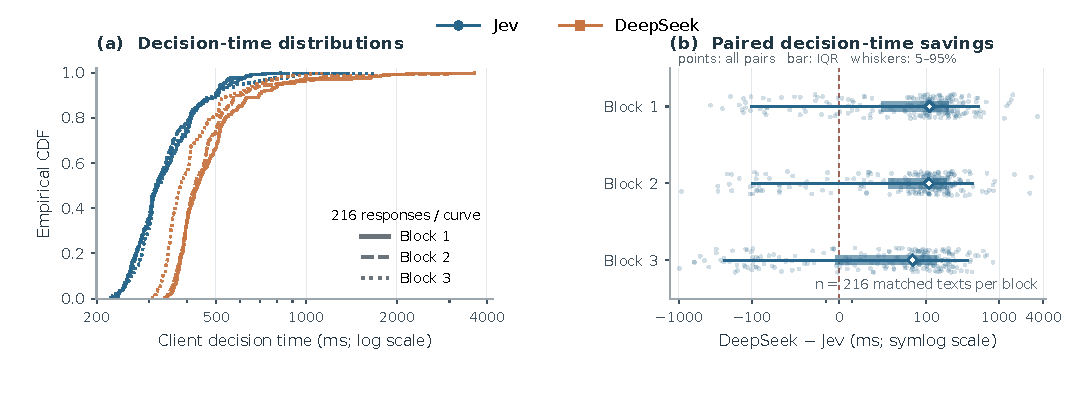
\includegraphics[width=\textwidth]{figures/decision-latency.pdf}
\caption{Study A decision latency on the same 216 texts per model and
consecutive block. (a) Full client response-time cumulative distribution
functions (CDFs) on a logarithmic time
axis. (b) All paired DeepSeek-minus-Jev differences: points, interquartile
bars, nearest-rank 5th--95th percentile whiskers, and median diamonds. The
symmetric-log axis is linear within $\pm50$\,ms. The ranges describe request
variation, not confidence intervals; texts recur across blocks.}
\label{fig:decision-latency}
\end{figure*}

Table~\ref{tab:quality} reports all three Study A blocks. Jev's median full
client decision time is 314.7--320.7\,ms, compared with DeepSeek's
381.4--434.7\,ms. The corresponding reductions are 26.5\%, 26.1\%, and
15.9\% in block order. Empirical p95 latency is also lower in each block,
by 36.7\%, 33.0\%, and 9.1\%, respectively. Jev's advantage varies across
the three blocks. Figure~\ref{fig:decision-latency} shows the full distributions
and their paired request-level differences.

\begin{table}[t]
\caption{Study A: exact four-field correctness and client decision latency.
Each row contains 216 requests; the same texts recur across blocks.}
\label{tab:quality}
\centering
% Generated by ../scripts/export_paper_draft_assets.py; do not hand-edit values.
\begin{tabular}{@{}clrrr@{}}
\toprule
Block & Backend & Correct & Median (ms) & p95 (ms) \\
\midrule
1 & Jev & 214/216 & 319.5 & 529.3 \\
1 & DeepSeek & 216/216 & 434.7 & 835.9 \\
2 & Jev & 213/216 & 314.7 & 557.8 \\
2 & DeepSeek & 215/216 & 425.9 & 833.2 \\
3 & Jev & 212/216 & 320.7 & 624.2 \\
3 & DeepSeek & 216/216 & 381.4 & 686.9 \\
\bottomrule
\end{tabular}

\end{table}

% Generated by scripts/plot_section_paper_results.py.
\begin{figure}[!tb]
\centering
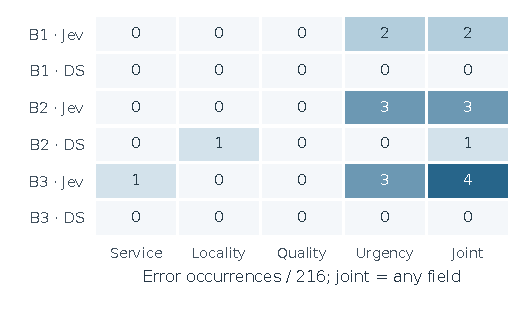
\includegraphics[width=\columnwidth]{figures/semantic-errors.pdf}
\caption{Study A semantic-error profile, with 216 responses per row.
Joint counts indicate an error in any field; B1--B3 are consecutive blocks
on reused texts, and DS denotes DeepSeek.}
\label{fig:semantic-errors}
\end{figure}


Both hosted APIs return schema-valid fields throughout Study A. DeepSeek
is more accurate on the strict semantic endpoint: it gets
216, 215, and 216 requests correct, versus Jev's 214, 213, and 212. Jev's
nine error occurrences span five distinct texts. Eight occurrences replace
unspecified urgency with normal urgency; the ninth maps an unsupported
recorded-speech translation request to OCR. This synthetic description
combines an unsupported translation intent with an image-transfer permission
clause. DeepSeek's single error replaces remote permission with unspecified
locality. Lower Jev decision latency therefore accompanies lower exact
semantic accuracy. Figure~\ref{fig:semantic-errors} resolves the errors by
field and block.

Operational equivalence explains why this semantic gap need not reduce
completion. Normal and unspecified urgency both map to ordinary
priority in this scheduler, so that field mismatch can leave execution
unchanged. In contrast, interpreting translation as OCR can dispatch the
wrong service. The latter text was not selected into Study A's execution
traces, so its effect is absent from the modeled completion results.

\subsection{Completion with Modeled Execution}
% Generated by scripts/plot_section_paper_results.py.
\begin{figure}[!tb]
\centering
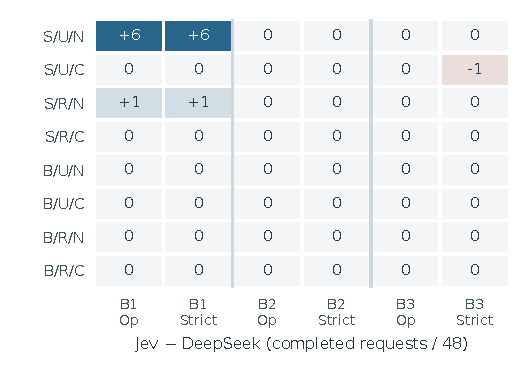
\includegraphics[width=\columnwidth]{figures/modeled-completion.pdf}
\caption{Study A completion differences across all 24 paired
conditions. Each cell is Jev minus DeepSeek, out of 48 arrivals. Op checks
operational requirements; Strict also requires exact field equality.
B1--B3 identify consecutive blocks. S/B denote steady/bursty arrivals, U/R changing/repeated text, and N/C cache off/on.}
\label{fig:modeled-completion}
\end{figure}

Across Study A's 24 paired conditions, Jev and DeepSeek have equal operational
completion counts in 22, and Jev has higher counts in two
(Fig.~\ref{fig:modeled-completion}). Summing the fixed matrix yields 884/884 supported
arrivals completed by Jev and 877/884 by DeepSeek. Each backend also receives
268 unsupported arrivals, which remain separate from execution successes.
The strict companion endpoint gives 21 ties, two conditions higher for Jev,
and one lower. In the latter condition, the loss is an unspecified-to-normal
urgency mismatch with the same executed priority, in a condition with no
cache hits.

% Generated by scripts/plot_section_paper_results.py.
\begin{figure*}[!t]
\centering
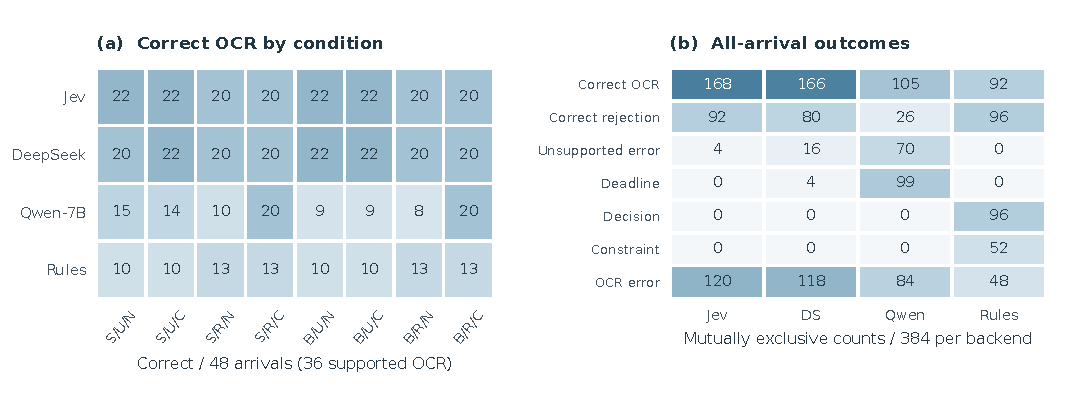
\includegraphics[width=\textwidth]{figures/ocr-outcomes.pdf}
\caption{Study B real-service outcomes, one run per condition and backend.
(a) Correct, on-time OCR completions in all 32 arms, each with 48 arrivals
and 36 supported requests. (b) Mutually exclusive outcomes among all 384
arrivals per backend; DS denotes DeepSeek. S/B denote steady/bursty arrivals, U/R changing/repeated text, and N/C cache off/on.}
\label{fig:ocr-outcomes}
\end{figure*}


Both operational gains occur in the first block without caching. In its
steady-changing condition, four DeepSeek calls take approximately
5.44--5.81\,s, and four additional arrivals expire while waiting. Six of
these eight failures are supported requests, yielding 36 Jev completions
versus 30 DeepSeek completions. In steady-repeated traffic, one supported
DeepSeek request lacks enough execution slack after waiting, yielding 41
versus 40 completions. These trajectories show how delayed decisions can
propagate into queueing and missed deadlines.

\subsection{Correct Completion in the Real OCR Service}

Table~\ref{tab:outcomes} aggregates the same eight conditions per backend.
Jev completes 168/288 supported requests correctly and on time (58.3\%),
versus 166/288 for DeepSeek (57.6\%). Qwen and rules complete 105/288 (36.5\%)
and 92/288 (31.9\%), respectively. Figure~\ref{fig:ocr-outcomes} retains all 384
arrivals per backend, including the 96 unsupported requests.

\begin{table}[t]
\caption{Study B: aggregate outcomes over eight conditions per backend.
Completed OCR and correctly rejected requests have different denominators.
False admissions count unsupported requests actually dispatched to OCR.}
\label{tab:outcomes}
\centering
% Generated by ../scripts/export_paper_draft_assets.py; do not hand-edit values.
\begin{tabular}{@{}lrrr@{}}
\toprule
Backend & Correct OCR & Correct rejection & False admit \\
\midrule
Jev & 168/288 & 92/96 & 4 \\
DeepSeek & 166/288 & 80/96 & 13 \\
Qwen2.5-7B & 105/288 & 26/96 & 4 \\
Rules & 92/288 & 96/96 & 0 \\
\bottomrule
\end{tabular}

\end{table}

Jev matches DeepSeek's correct-completion count in seven conditions and
exceeds it by two in one (Table~\ref{tab:paired}). Service-output errors
remain substantial: the outcome breakdown
attributes 120 Jev arrivals and 118 DeepSeek arrivals to OCR content or
execution failure, after preceding failure categories have been excluded.
Checking the returned text exposes these failures even when the decision
and service calls themselves succeed.

Among unsupported requests, Jev correctly rejects
92/96 and dispatches four unsupported requests to OCR. All four are repeated
occurrences of one translation intent across conditions. DeepSeek correctly
rejects 80/96, with 13 actual false
admissions; the remaining three mishandled unsupported requests do not result
in an OCR dispatch. Rules reject all 96 unsupported requests, but also lose
supported jobs through interpretation and execution-constraint failures.
No forbidden off-site image bytes are observed for any backend in these
runs, which include 22 remote executions for Jev and 30 for DeepSeek.

\begin{table*}[!t]
\caption{Study B: all Jev--DeepSeek paired conditions. Each condition has 48
arrivals, of which 36 require OCR. Completion counts retain all failures;
latencies use only the $N$ requests completed correctly by both backends.
Positive paired saving means faster completion with Jev.}
\label{tab:paired}
\centering
% Generated by ../scripts/export_paper_draft_assets.py; do not hand-edit values.
\begin{tabular}{@{}lllrrrrrr@{}}
\toprule
 & & & \multicolumn{2}{c}{Correct completions} & & \multicolumn{2}{c}{Median full time (ms)} & Median paired \\
\cmidrule(lr){4-5}\cmidrule(lr){7-8}
Load & Description & Cache & Jev & DeepSeek & $N$ & Jev & DeepSeek & saving (ms) \\
\midrule
Steady & Changing & Off & 22 & 20 & 20 & 410.4 & 538.6 & 135.69 \\
Steady & Changing & On & 22 & 22 & 22 & 418.3 & 483.1 & 84.93 \\
Steady & Repeated & Off & 20 & 20 & 20 & 436.4 & 490.8 & 70.63 \\
Steady & Repeated & On & 20 & 20 & 20 & 110.9 & 112.4 & -0.37 \\
Bursty & Changing & Off & 22 & 22 & 22 & 438.7 & 587.6 & 101.14 \\
Bursty & Changing & On & 22 & 22 & 22 & 478.2 & 515.2 & 74.43 \\
Bursty & Repeated & Off & 20 & 20 & 20 & 436.3 & 555.5 & 125.86 \\
Bursty & Repeated & On & 20 & 20 & 20 & 106.2 & 109.0 & -0.49 \\
\bottomrule
\end{tabular}

\end{table*}

\subsection{End-to-End Latency and the Cache Boundary}
% Generated by scripts/plot_section_paper_results.py.
\begin{figure}[!tb]
\centering
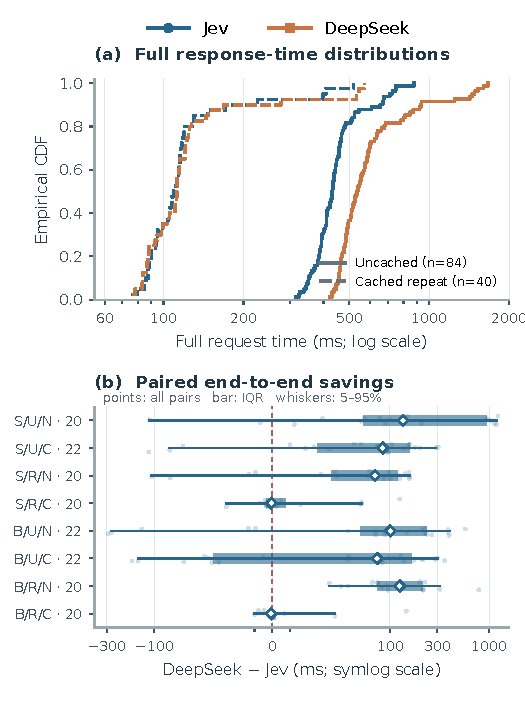
\includegraphics[width=\columnwidth]{figures/ocr-latency.pdf}
\caption{Study B latency on requests completed correctly by both
Jev and DeepSeek. (a) Descriptive pooled CDFs; sample size $n$ is 84 per model
for the four uncached conditions and 40 for the two repeated-text cached
conditions. Changing-text cached arms are excluded from this panel.
(b) Every paired difference in all eight conditions; row suffixes give $n$.
Bars show the interquartile range, whiskers the nearest-rank 5th--95th
percentiles, and diamonds the median. The symmetric-log axis is linear
within $\pm50$\,ms. Ranges are descriptive, not confidence intervals.
S/B denote steady/bursty arrivals, U/R changing/repeated text, and N/C cache off/on.}
\label{fig:ocr-latency}
\end{figure}

On the common-success subset, Jev reduces median full request latency by
11.1--25.3\% in the four cache-disabled conditions. These comparisons contain
20 or 22 paired successful requests each. Median per-request savings range
from 70.6 to 135.7\,ms (Table~\ref{tab:paired}). These durations include
image transfer, worker queueing, OCR execution, and response delivery.

% Generated by scripts/plot_section_paper_results.py.
\begin{figure}[!tb]
\centering
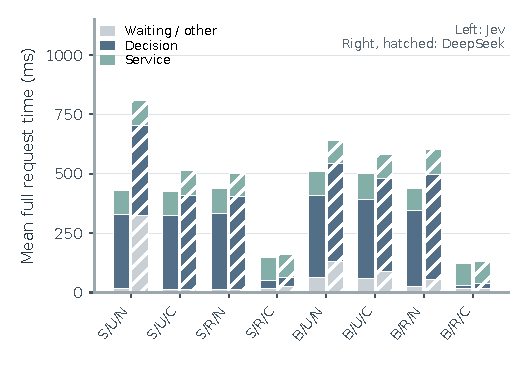
\includegraphics[width=\columnwidth]{figures/ocr-time-components.pdf}
\caption{Study B mean time composition on each condition's
common-success subset. The service component includes transfer and OCR; the residual
includes queueing and controller handling. Left bars are Jev; right,
hatched bars are DeepSeek. Components sum to the arithmetic mean, not the
median. S/B denote steady/bursty arrivals, U/R changing/repeated text, and N/C cache off/on.}
\label{fig:ocr-time-components}
\end{figure}


Figure~\ref{fig:ocr-latency}b retains every paired latency difference, including
requests on which DeepSeek is faster. Figure~\ref{fig:ocr-time-components}
decomposes mean full time on the same successful subsets. Its service component includes
image transfer and OCR; the remaining time includes controller handling and
queueing.

Caching changes the result when descriptions repeat. With caching enabled,
the steady-repeated medians are 110.9\,ms for Jev and 112.4\,ms for DeepSeek;
the bursty-repeated medians are 106.2 and 109.0\,ms. Yet the median paired
savings are $-0.37$ and $-0.49$\,ms, respectively. The small opposite signs
arise because a difference of marginal medians is not a median of paired
differences. Neither comparison supports a material latency advantage after
the reusable decisions are cached. Figure~\ref{fig:ocr-latency}a also contrasts
the uncached and repeated-text cached response-time distributions. Changing-text conditions have no exact
cache hits; differences between their cache-on and cache-off arms reflect
separate executions, not a benefit from cache lookup.

Qwen has
105 correct completions in the full matrix and 99 arrivals classified as
deadline or infeasibility failures. Its conditional median model-call time
is 1.408\,s, consuming a substantial part of the request budget before
service execution.
The called request subsets differ across backends because of cache hits and
expiry, so this conditional median is diagnostic rather than a paired
model-speed benchmark. With repeated-text caching, Qwen reaches 20 correct
completions in both load conditions, matching the hosted backends there.

\subsection{Billed API Cost}
% Generated by scripts/plot_section_paper_results.py.
\begin{figure}[!tb]
\centering
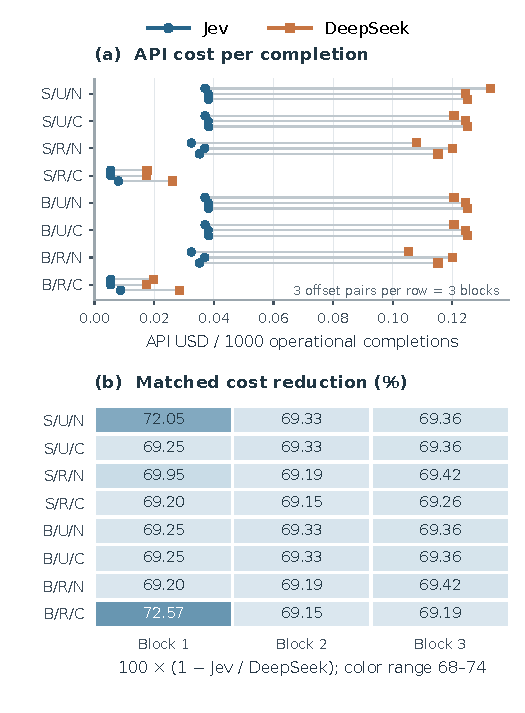
\includegraphics[width=\columnwidth]{figures/modeled-api-cost.pdf}
\caption{Study A billed API cost per modeled operational completion.
(a) Absolute fees, scaled to 1000 completions; top-to-bottom offsets within
each row distinguish blocks 1--3. (b) Matched reductions, with color range
68--74\%. Fees include all trajectory calls and exclude warmups and
separate quality evaluation. S/B denote steady/bursty arrivals, U/R changing/repeated text, and N/C cache off/on.}
\label{fig:modeled-api-cost}
\end{figure}

Study A's API fees per operational completion are 69.15--72.57\% lower
with Jev across the 24 pairs (Fig.~\ref{fig:modeled-api-cost}). These costs
include unsuccessful requests and use observed modeled completion counts.
The absolute fees and matched reductions retain all three blocks separately.

% Generated by scripts/plot_section_paper_results.py.
\begin{figure}[!tb]
\centering
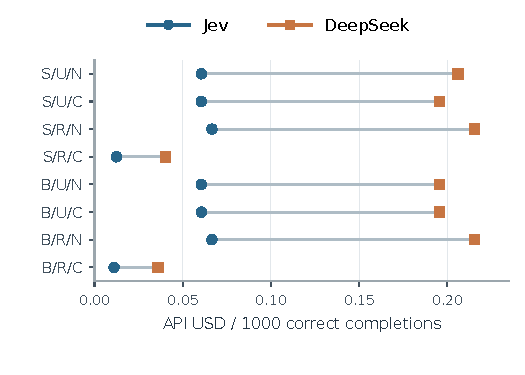
\includegraphics[width=\columnwidth]{figures/ocr-api-cost.pdf}
\caption{Study B API fees per correct OCR completion, scaled to
1000. Charges include all trajectory calls, including unsuccessful
requests, but exclude warmups, computation, network, and other operating
costs. S/B denote steady/bursty arrivals, U/R changing/repeated text, and N/C cache off/on.}
\label{fig:ocr-api-cost}
\end{figure}

Jev's API fees per correct OCR completion are 68.97--70.61\% lower over all
eight paired conditions; the cache-disabled range is 69.03--70.61\%.
Depending on the condition, the observed values scale to approximately
\$0.011--\$0.067 per 1000 correct completions for Jev, versus
\$0.036--\$0.215 for DeepSeek (Fig.~\ref{fig:ocr-api-cost}).

Caching reduces the absolute fee for both models and leaves a similar
relative API-cost gap on the remaining calls.

\section{Discussion}
\subsection{Implications for Service Orchestration}
The experiments show a practical use for Jev in edge-service admission:
reducing the time and API fees spent interpreting requests while retaining
the observed correct-completion counts. The shared intent contract lets
Jev replace the generative interpreter within the same validation and
scheduling pipeline. The real OCR results show that the latency benefit
remains visible after image transfer, worker queueing, and recognition.

This integration gives service designers two ways to reduce interpretation
overhead. A faster decision backend shortens fresh calls, while caching
reuses decisions for repeated descriptions. The repeated-text conditions
show how effective the latter can be, including for self-hosted Qwen.
Choosing between backends therefore depends on the share of requests that
need a new decision and the time available for service execution. In the
admission path studied here, shorter decision waiting leaves more deadline
slack and releases interpretation capacity sooner.

\subsection{Evaluating the Complete Service Path}
The shared scheduler connects interpreter performance to delivered service.
It reads current worker state after interpretation and checks placement,
tier, priority, and predicted completion time before dispatch. Evaluating
intent fidelity, execution compliance, and actual output separately makes
it possible to trace how an interpretation affects the final result.
For example, the normal-versus-unspecified urgency difference maps to the
same execution priority, while the returned OCR text determines whether
recognition succeeded. This evaluation supports a service-level choice of
interpreter using completion, response time, and fees together.

\subsection{Scope and Next Steps}
The studies use synthetic English requests, repeated texts and images, and
one measurement session; completion retention is descriptive as defined in
Section~\ref{sec:design}. The real service has two workers and one service
family. Hosted timings include provider and network paths, with sequential
runs exposed to temporal variation. They compare deployed services rather
than isolate internal model inference. API fees cover interpretation calls;
local compute and communication costs are outside this measure.
Appendix~\ref{app:settings} records the configuration.

The next step is to evaluate independently authored requests across days,
services, and network conditions, using deadlines drawn from application
requirements. Optimized local serving and a domain-trained classifier or
bounded extractor, absent from the present comparison, would extend the
available deployment choices.

\section{Conclusion}
We integrated Jev into an edge-service admission pipeline and evaluated its
ability to replace a concise generative interpreter. The shared contract
and scheduler connect decision latency to actual service completion. Across
three measurement blocks, Jev reduces median decision latency by
15.9--26.5\%. In the real OCR service, it matches or exceeds DeepSeek's
correct-completion count in all eight paired conditions. Median response
time among shared successes is 11.1--25.3\% lower without caching. Across
all eight conditions, API fees per correct completion are 69.0--70.6\% lower.
These results support Jev as a practical alternative for the tested
admission workload. Faster decisions address requests that need fresh
interpretation, while caching reuses decisions for repeated descriptions.


\bibliographystyle{IEEEtran}
\bibliography{references}
\appendices
\section{Implementation and Evaluation Settings}
\label{app:settings}
\subsection{Interpretation Backends}
The studies were executed on September 18, 2026. Jev uses OpenRouter's
Decisions endpoint with identifier typesafe/jev-1.13; responses identify
jev-1.13-20260917 and provider TypeSafe. Four native Choice questions return
the shared intent fields in one request. DeepSeek uses deepseek-v4.1-flash
through OpenRouter, pinned to Together with provider fallback disabled.
It returns a strict four-field JSON object with temperature zero, a
128-token limit, and reasoning disabled; recorded reasoning-token counts
are zero.

Qwen2.5-7B-Instruct, revision a09a35458c70, runs in brain floating point 16
(BF16) on one NVIDIA L40, using Transformers with scaled dot-product
attention (SDPA) and PyTorch 2.2.0+cu121. It uses the same generative prompt
and field contract as DeepSeek, greedy decoding, and a 128-token limit.
The server batches up to four already-pending requests without an intentional
collection delay. The fixed rule parser uses keywords and regular expressions
without tuning on evaluation wording.

\subsection{Admission and Execution Controls}
Both studies use a 2\,s request deadline, four concurrent interpretation
slots, and an admission queue of capacity 32. API calls have a 15\,s timeout,
with no automatic retries or repair calls. Connections are warmed before
measurement. Each condition starts with an empty cache keyed by normalized
full request text and extraction policy. The controller checks it before
queueing and after obtaining a slot; concurrent misses are not coalesced.

The real service has one local macOS worker and one remote Linux worker,
connected through a Secure Shell (SSH) tunnel. The remote allocation provides
six processor cores and the accelerator used by Qwen; OCR uses processors
only. Each node has one nonpreemptive worker and a queue of capacity 16.
Urgent and ordinary jobs have priority values zero and one, respectively;
equal-priority jobs follow enqueue order. The controller verifies the returned
node, tier, priority, and image identity. A timed-out OCR process is terminated
before capacity is released. Transport or protocol errors stop further calls.
The recorded environment lacks a complete processor inventory for exact
cross-site reproduction.

\subsection{Study A Parameters}
The 216 requests use six wording families and two instances of each of the
108 field combinations, with extraction instructions held fixed. Seeds 42,
43, and 44 vary request order and arrival traces across three consecutive
blocks. Each model has 648 semantic measurements on the same 216 texts.
There is one semantic-stage warmup per model per block and no fixed interval
between blocks.

Each service condition has 48 arrivals. Steady traffic has rate 2 requests/s;
bursty traffic alternates 0.5 and 8 requests/s in 20\,s segments. The execution
model has four edge nodes and one cloud node, with payloads of 0.25--2\,MB.
Local, other-edge, and cloud links have propagation delays of 2, 20, and
60\,ms and bandwidths of 1000, 100, and 50\,Mbit/s, respectively; transfer
also includes serialization. Base durations are 40\,ms for counting, 80\,ms
for detection, and 60\,ms for OCR. The high tier multiplies these by 1.8;
node factors are 1.0, 1.1, 1.2, and 1.3 for the edges and 0.65 for the cloud.
Each node has one priority worker. These are exploratory simulation inputs.

\subsection{Study B Parameters and Scoring}
Model conditions run sequentially in randomized order with seed 42 and no
fixed cooldown. Both workers use Tesseract 5.5.3, English recognition,
one OpenMP thread, and single-word mode (engine mode 1, segmentation mode 8).
Standard and high tiers use tessdata\_fast and tessdata\_best, respectively,
with identical weights across nodes. Seed 42 selects 20 training and 80 test
images from sorted IIIT5K identifiers before recognition outcomes are known.

Calibration runs each training image once per node and tier. Median
request--response durations, including transfer, are 80.85/96.26\,ms for
local standard/high and 95.30/139.35\,ms for remote standard/high.
The workload has 48 distinct intents. Repeated-text conditions use eight
descriptions, six supported and two unsupported, each repeated six times.
The test images recur across conditions. Arrival rates match Study A;
eight conditions for four backends produce 32 runs and 1536 arrivals.

OCR comparison uses case-preserving character annotations without a
recognition lexicon, normalizes Unicode to Normalization Form C (NFC), and
strips surrounding whitespace. Quantile summaries use nearest-rank 5th and
95th percentiles and linearly interpolated interquartile ranges. Each
request is evaluated on its recorded timing and output; cached decisions
do not replace service execution.

\end{document}
